\documentclass[10pt]{beamer}
\usetheme[
%%% options passed to the outer theme
%    hidetitle,           % hide the (short) title in the sidebar
%    hideauthor,          % hide the (short) author in the sidebar
%    hideinstitute,       % hide the (short) institute in the bottom of the sidebar
%    shownavsym,          % show the navigation symbols
%    width=2cm,           % width of the sidebar (default is 2 cm)
%    hideothersubsections,% hide all subsections but the subsections in the current section
%    hideallsubsections,  % hide all subsections
    left               % right of left position of sidebar (default is right)
%%% options passed to the color theme
%    lightheaderbg,       % use a light header background
  ]{AAUsidebar}

% If you want to change the colors of the various elements in the theme, edit and uncomment the following lines
% Change the bar and sidebar colors:
%\setbeamercolor{AAUsidebar}{fg=red!20,bg=red}
%\setbeamercolor{sidebar}{bg=red!20}
% Change the color of the structural elements:
%\setbeamercolor{structure}{fg=red}
% Change the frame title text color:
%\setbeamercolor{frametitle}{fg=blue}
% Change the normal text color background:
%\setbeamercolor{normal text}{bg=gray!10}
% ... and you can of course change a lot more - see the beamer user manual.

\usepackage{blkarray}

\usepackage[utf8]{inputenc}
\usepackage[english]{babel}
\usepackage[T1]{fontenc}
% Or whatever. Note that the encoding and the font should match. If T1
% does not look nice, try deleting the line with the fontenc.
\usepackage{helvet}
\usepackage{tikz}                  % drawing vector graphics
\usepackage{circuitikz}            % drawing circuits
\usepackage{mathtools}
%laplace
\usepackage{mathrsfs}
\usepackage{siunitx}    % si-units
\usepackage{amssymb}

%Bibliography
\usepackage[square]{natbib}

\usepackage{tikz}
\usepackage{circuitikz}
\usepackage{graphicx}
\usepackage{caption}
\usepackage{physics}
\usepackage{subcaption}
\usepackage{stackengine}
\usepackage{media9}
\usepackage{multimedia}
\mathtoolsset{showonlyrefs}
\usepackage{pgfplots}

\usetikzlibrary{arrows.meta}
\usetikzlibrary{positioning,calc}
\usetikzlibrary{intersections}
\usetikzlibrary{shapes.misc}
\tikzset{>={Latex[width=1mm,length=1.2mm]},
  Speaker/.pic={
    \filldraw[fill=gray!40,pic actions] 
    (-15pt,0) -- 
      coordinate[midway] (-front) 
    (15pt,0) -- 
    ++([shift={(-6pt,8pt)}]0pt,0pt) coordinate (aux1) -- 
    ++(-18pt,0) coordinate (aux2) 
    -- cycle 
    (aux1) -- ++(0,6pt) -- coordinate[midway] (-back) ++(-18pt,0) -- (aux2);
  },cross/.style={cross out, draw=black, minimum size=2*(#1-\pgflinewidth), inner sep=0pt, outer sep=0pt},cross/.default={1pt},
  Box/.pic={
  \draw (0,0) to (0.5,0) to (0.5,-1) to (0.5,-1) to (-.5,-1) to (-.5,0) to (0,0);
  },
  Sbox/.pic={
  \draw (0,0) to (0,0.5) to (1.5,0.5) to (1.5,-0.5) to (0,-0.5) to (0,0);
  },
  Vbox/.pic={
  \draw (0,0) to (1.5,0) to (1.5,-1) to (-1.5,-1) to (-1.5,0) to (0,0);
  },
  variables/.pic={
  \draw (0,0) to (0,0.5) to (1.5,0.5) to (1.5,-0.5) to (0,-0.5) to (0,0);
  \draw (0,0) to (1.5,0);
  },
  pics/microphone/.style={code={ 
        \draw[black, line width=.2em, rounded corners=1.7ex] 
            (-.85em,4.5ex) -- (-.85em,2ex) -- (.85em,2ex) -- (.85em,4.5ex);
        \fill[black] 
            (-.6em,5ex) to[rounded corners=1.2ex]  
            (-.6em,2.5ex) to[rounded corners=1.2ex] (.6em,2.5ex)
            -- (.6em,5ex) to[rounded corners=.2ex] ++(-.85em,0) to[rounded corners=.2ex] ++(0,.35ex) -- ++(.85em,0)  
            -- (.6em,5.5ex) to[rounded corners=.2ex] ++(-.85em,0) to[rounded corners=.2ex] ++(0,.35ex) -- ++(.85em,0)
            -- (.6em,6ex) to[rounded corners=.2ex] ++(-.85em,0) to[rounded corners=.2ex] ++(0,.35ex) -- ++(.85em,0)
            -- (.6em,6.5ex) to[rounded corners=.2ex] ++(-.85em,0) to[rounded corners=.2ex] ++(0,.35ex) -- ++(.85em,0)
            to[rounded corners=1.2ex]
            (.6em,8ex) to[rounded corners=1.2ex]
            (-.6em,8ex) to[rounded corners=1.2ex] cycle; 
        \fill[black] (-.1em,1.8ex) rectangle (.1em,.5ex);
        \fill[black] (-.5em,.5ex) rectangle (.5em,0);
    }}}

% colored hyperlinks
\newcommand{\chref}[2]{%
  \href{#1}{{\usebeamercolor[bg]{AAUsidebar}#2}}%
}
\tikzstyle{point} = [fill,shape=circle,minimum size=3pt,inner sep=0pt]
\tikzstyle{edge} = [fill=white,midway,inner sep=1pt]



\title[P2]% optional, use only with long paper titles
{Lineær programmeringsproblemer}

\subtitle{Simplexmetoden}  % could also be a conference name

\date{29. Juni 2020}

\author[Gruppe B303c] % optional, use only with lots of authors
{
	Jens Koldkur				\\
	Jonas Bach Christensen		\\
	Julie Havbo Lund			\\
	Mads Bjerregaard Kjær		\\
	Mathias Gammelgaard			\\
	Rasmus Jespersgaard
}
% - Give the names in the same order as they appear in the paper.
% - Use the \inst{?} command only if the authors have different
%   affiliation. See the beamer manual for an example

\institute[
%  {\includegraphics[scale=0.2]{aau_segl}}\\ %insert a company, department or university logo
%  Dept.\ of Mathematical Sciences\\
%  Skjernvej 4A\\
%  DK-9220 Aalborg Ø
] % optional - is placed in the bottom of the sidebar on every slide
{% is placed on the title page
%  Dept.\ of Mathematical Sciences\\
%  Skjernvej 4A\\
%  DK-9220 Aalborg Ø
  
  %there must be an empty line above this line - otherwise some unwanted space is added between the university and the country (I do not know why;( )
}


% specify a logo on the titlepage (you can specify additional logos an include them in 
% institute command below
\pgfdeclareimage[height=1.5cm]{titlepagelogo}{AAUgraphics/aau_logo_new} % placed on the title page
%\pgfdeclareimage[height=1.5cm]{titlepagelogo2}{graphics/aau_logo_new} % placed on the title page
\titlegraphic{% is placed on the bottom of the title page
  \pgfuseimage{titlepagelogo}
%  \hspace{1cm}\pgfuseimage{titlepagelogo2}
}

% Sets
\newcommand{\N}{\mathbb{N}}  % natural numbers
\newcommand{\Z}{\mathbb{Z}}  % integers
\newcommand{\Q}{\mathbb{Q}}  % rational numbers
\newcommand{\R}{\mathbb{R}}  % real numbers
\newcommand{\C}{\mathbb{C}}  % complex numbers
\newcommand{\I}{\mathbb{I}}  % imaginary numbers
\renewcommand{\b}[1]{\mathbf{#1}}
\renewcommand{\L}{\mathcal{L}}
\newcommand{\U}{\mathcal{U}}
\newcommand{\Y}{\mathcal{Y}}
\newcommand{\B}{\mathcal{B}}

% Colors 
\definecolor{AAUblue1}{RGB}{ 33, 26, 82}
\definecolor{AAUblue2}{RGB}{ 89, 79,191}
\definecolor{AAUgrey1}{RGB}{ 84, 97,110}
\definecolor{AAUgrey2}{RGB}{104,119,132}
\definecolor{AAUgrey3}{RGB}{162,172,182}
\definecolor{AAUgrey4}{RGB}{222,223,226}
\definecolor{AAUgreen}{RGB}{157,187, 29}
\definecolor{AAUteal} {RGB}{ 94,150,149}
\definecolor{AAUred}  {RGB}{223,103, 82}
%farvet-commands
\definecolor{myblue}{RGB}{89, 79, 191}
\definecolor{mygreen}{RGB}{157, 187, 29}
\definecolor{myred}{RGB}{223, 103, 82}
\definecolor{mygrey}{RGB}{222, 223, 226}
\usepgfplotslibrary{fillbetween}


% Semantics
\let\cross=\times
\let\times=\cdot
\newcommand{\euler}{e}%\mathfrak{e}}
\renewcommand{\exp}[1]{\euler^{#1}}
\renewcommand{\matrix}[1]{\begin{bmatrix}#1\end{bmatrix}}
\newcommand{\amatrix}[2]{\left[\begin{array}{@{}*{#1}{c}|c@{}}#2\end{array}\right]}
\renewcommand{\vec}[1]{\mathrm{\mathbf{#1}}}
\newcommand{\transpose}{^\intercal}
% \newcommand{\dotproduct}{\boldsymbol{\cdot}}
\newcommand{\dotp}{\dotproduct}
\newcommand{\directsum}{\oplus}
\newcommand{\cardinality}[1]{\mathit{card}\bigl({#1}\bigr)}
\newcommand\oast{\stackMath\mathbin{\stackinset{c}{0ex}{c}{0ex}{\ast}{\bigcirc}}}

% Other operators and concepts
\newcommand{\bigO}{\mathcal{O}}                                             % big O
\renewcommand\qedsymbol{$\blacksquare$}                                     % use black square as QED
\DeclarePairedDelimiterXPP{\laplace}[1]{\mathscr{L}}{\{}{\}}{}{#1}          % Laplace transform
\DeclarePairedDelimiterXPP{\invlaplace}[1]{\mathscr{L}^{-1}}{\{}{\}}{}{#1}  % Inverse laplace transform
\DeclarePairedDelimiterXPP{\fourier}[1]{\mathscr{F}}{\{}{\}}{}{#1}          % Fourier transform
\DeclarePairedDelimiterXPP{\invfourier}[1]{\mathscr{F}^{-1}}{\{}{\}}{}{#1}  % Inverse fourier transform

\begin{document}
% the titlepage
{\aauwavesbg%
\begin{frame}[plain,noframenumbering] % the plain option removes the sidebar and header from the title page
  \titlepage
\end{frame}}
%%%%%%%%%%%%%%%%

% TOC
\begin{frame}{Disposition}{}
\tableofcontents
\end{frame}
%%%%%%%%%%%%%%%%

\section{Lineær algebra}
\begin{frame}
\centering
\Huge
Lineær algebra
\end{frame}
%
\begin{frame}
\frametitle{Lineær Algebra}
\begin{itemize}
\item \textbf{$nr. 1$}
\item Matrixsum og skalering.
\item Transponering.
\item Matrix-vektorprodukt og matrixmultiplikation.
\item Linearkombinationer.
\item Span.
\item Lineær uafhængighed.
\item Underrum.
%Kort om Matrixsum og skalering, Transponering Matrix-vektorprodukt og matrixmultiplakation.
\end{itemize}
\end{frame}
%%
\section{Lineære ligningssystemer}
\begin{frame}
\centering
\Huge
Lineære ligningssystemer
\end{frame}
%
\begin{frame}
\frametitle{Lineære ligningssystemer}
\begin{itemize}
\item Et system af $m$ lineære ligninger med de samme $n$ variable. 
\item Eksempel:
\begin{align*}
x_1-x_3-2x_4-8x_5&=-3 \\
-2x_1+x_3+2x_4+9x_5&=5 \\
3x_1-2x_3-3x_4-15x_5&=-9.
\end{align*}
\item Ingen, én eller uendeligt mange løsninger. 
\item Hvis systemet ingen løsning har, er det inkonsistent. Ellers er det konsistent. 
\end{itemize}
\end{frame}
%%
\begin{frame}
\frametitle{Lineære ligningssystemer}
\begin{itemize}
\item Lineære ligningssystemer kan opstilles i en totalmatrix. 
\item Totalmatricen er koefficientmatricen udvidet. 
\item Eksempel:
\begin{equation*}
  [A \mid \mathbf{b}] =
\begin{blockarray}{ccccccc}
x_1 & x_2 & x_3 & x_4 & x_5 & b \\
\begin{block}{[ccccc|c]c}
  1 & 0 & -1 & -2 & -8 & -3 \\
  -2 & 0 & 1 & 2 & 9 & 5 \\
  3 & 0 & -2 & -3 & -15 & -9 \\
\end{block}
\end{blockarray}.
\end{equation*}
\item Løsningen er en vektor \mathbf{v}, således at ligningerne er opfyldt, når $x_i = v_i$.
\end{itemize}
\end{frame}
%%
\begin{frame}
\frametitle{Rækkeoperationer}
\begin{itemize}
\item Totalmatricen gør det let at udføre elementære rækkeoperationer. 
\item Ombytning: $A \xrightarrow{R_i \leftrightarrow R_j} B$. 
\item Skalering: $A \xrightarrow{R_i \rightarrow cR_i} B$.
\item Udskiftning: $A \xrightarrow{R_i \rightarrow R_i + cR_h} B$.
\end{itemize}
\end{frame}
%%
\begin{frame}
\frametitle{Trappeform}
\begin{itemize}
\item Kan opnås via elementære rækkeoperationer. 
\item Ikke-nulrækker over nulrækker. 
\item Første ikke-nulindgang ligger i en søjle til højre for ikke-nulindgangen i forrige række. 
\item Hvis en søjle har den første ikke-nulindgang i en række, er alle understående indgange i søjlen nulindgange. 
\item Eksempel: 
\begin{align*}
A=
\begin{blockarray}{cccc}
\begin{block}{[cccc]}
2 & 4 & 8 & 2\\
0 & 5 & -2 & 5\\
0 & 0 & 2 & 7\\
0 & 0 & 0 & 0\\
\end{block}
\end{blockarray}
\text{ og }
B=
\begin{blockarray}{cccc}
\begin{block}{[cccc]}
2 & 4 & 8 & 2\\
0 & 0 & -2 & 5\\
0 & 4 & 2 & 7\\
0 & 0 & 0 & 4\\
\end{block}
\end{blockarray}.
\end{align*}
\end{itemize}
\end{frame}
%%
\begin{frame}
\frametitle{Reduceret trappeform}
\begin{itemize}
\item Kan opnås via elementære rækkeoperationer. 
\item Matricen er på trappeform.
\item Hvis en søjle har den første ikke-nulindgang i en række, så er alle øvrige indgange i søjlen $0$.
\item Den første ikke-nulindgang i hver ikke-nulrække er lig $1$. 
\item Eksempel: 
\begin{align*}
A_R=
\begin{blockarray}{ccccc}
\begin{block}{[ccccc]}
1 & 0 & 5 & 0 & 0\\
0 & 1 & 3 & 0 & 0\\
0 & 0 & 0 & 1 & 0\\
0 & 0 & 0 & 0 & 1\\
\end{block}
\end{blockarray}
\end{align*}
\item Konsistens og pivot. 
\end{itemize}
\end{frame}
%%
\begin{frame}
\frametitle{Gauss-elimination}
\begin{itemize}
\item En algoritme, der benytter elementære rækkeoperationer. 
\item Reducerer en matrix til reduceret trappeform. 
\end{itemize}
\begin{enumerate}
\item Find første ikke-nulsøjle fra venstre i matricen.
\item Ved rækkeombytning placeres en ikke-nulindgang øverst i pivotsøjlen.
\item Skab nulindgange under pivotindgangen ved hjælp af rækkeudskiftning.
\item Øverste række markeres som afsluttet og trin $1-4$, hvor afsluttede rækker ignoreres.
Dette gentages, indtil alle rækker er markeret som afsluttet.
\item Alle rækker med pivotindgange skaleres, så alle pivotindgange er lig $1$.
\item Ved rækkeudskiftning sikres nu nulindgange over og under pivotindgangene.
\end{enumerate}
\end{frame}
%%
\begin{frame}
\frametitle{Rang og nullitet}
\begin{itemize}
\item Rang$(A)$ er antallet af pivotsøjler i en matrix $A$. 
\item Null$(A)$ er antallet er ikke-pivotsøjler i en matrix $A$. 
\item I en $m \cross n$ matrix er Rang$(A)$ $+$ Null$(A) = n$. 
% Kort!!
\end{itemize}
\end{frame}
\section{Løsninger af lineære optimeringsproblemer}
%
\begin{frame}
\centering
\Huge
Løsning af lineære optimeringsproblemer 
\end{frame}
%
%\begin{frame}
%\frametitle{Løsning af lineære \phantom{HHHHHHHHHHHH} optimeringsproblemer}
%\begin{itemize}
%\item \textbf{$nr. 3$}
%\item Intro til løsninger fra afsnit 2
%%De fire punkter fra raporten (angående løsninger)
%\item Standardform.
%\item Eventuelt dualproblemer som sidebemærkning. Hvis vi skal have det med måske en bemærkning om spilteori og nulsum(slackvariable løsning for dual).
%\item Polyedre og repræsentation(herunder standardform)
%\item Det konvekse hylster.
%\item Lokal $\rightarrow$ Global (omkring fig 3.9)
%\end{itemize}
%\end{frame}

\begin{frame}
\frametitle{Optimeringsproblemer}
\begin{align*}
\begin{array}{lrll}
\text{Maksimér}		&\textbf{c}^T\textbf{x}	& = z		&\\
\text{begrænset af}	&\textbf{a}^T\textbf{x}	&\geq b_i,	&i \in M_1,\\
					&\textbf{a}^T\textbf{x}	&\leq b_i,	&i \in M_2,\\
					&\textbf{a}^T\textbf{x}	& = b_i,	&i \in M_3,\\
					&x_j					&\geq 0,	&j \in N_1,\\
					&x_j					&\leq 0,	&j \in N_2,
\end{array}
\end{align*}
\begin{itemize}
\item Objektfunktionen
\item Lineære betingelser 
\item Fra min til maks 
\begin{itemize}
\item -1 
\item Ulighed fra $\textbf{A}_i \textbf{x} \geq b_i$ til $-\textbf{A}_i \textbf{x} \leq -b_i$
\end{itemize}
\end{itemize}
\end{frame}

\begin{frame}
\frametitle{Grafisk løsning}
\begin{figure}[H]
\centering
%
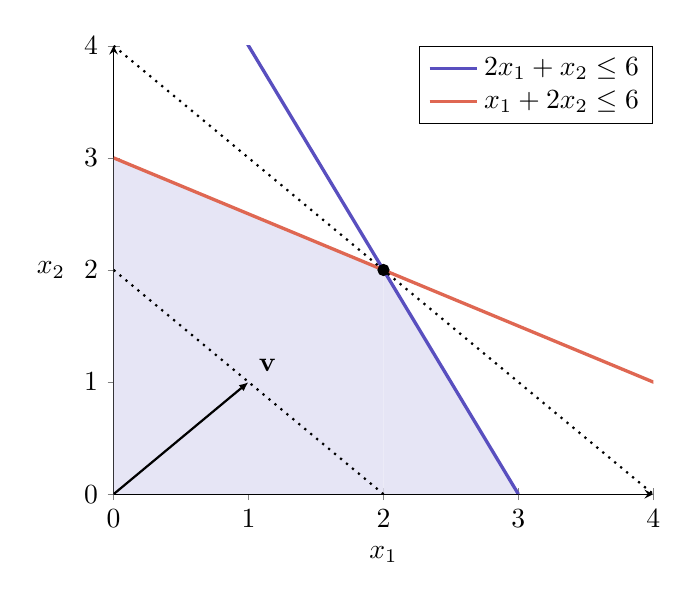
\begin{tikzpicture}%[scale=0.5]
%
%
% -------------------------------------------------------
\begin{axis}[
axis lines = left,
	xlabel = $x_1$,
	ylabel = \rotatebox{-90}{$x_2$},
  xmax=4,
  ymax=4,
	legend style={at={(1,1)},anchor=north east},
]
%%%
%%%
\addplot[name path=b, domain={0:3}, color=myblue, style=very thick,samples=2]{6-2*x};
\addlegendentry{$2x_1+x_2 \leq 6$}
\addplot[name path=a, domain={0:6}, color=myred, style=very thick, samples=2]{3-0.5*x};
\addlegendentry{$x_1+2x_2 \leq 6$}
%
\addplot[name path=c, domain=0:3,samples=2,color=black, style=very thin]{0};
%
\addplot[fill=myblue!15] fill between [of=a and c, soft clip={domain=0:2}];
\addplot[fill=myblue!15] fill between [of=b and c, soft clip={domain=2:3}];
%
%
%	
\addplot[domain=0:6, samples=2, color=black, dotted, thick]{-x};
\addplot[domain=0:6, samples=2, color=black, dotted, thick]{2-x};
\addplot[domain=0:6, samples=2, color=black, dotted, thick]{4-x};
\addplot[mark=*] coordinates {(2,2)};
\addplot[mark=none] coordinates {(0,0) (0,3)};
\addplot[mark=none, thick, ->] coordinates {(0,0) (1,1)} node[above right] {$\mathbf{v}$};
\end{axis}
\end{tikzpicture}
\end{figure}
\end{frame}

\begin{frame}
\frametitle{Grafisk løsning}
\begin{figure}[H]
\centering
%
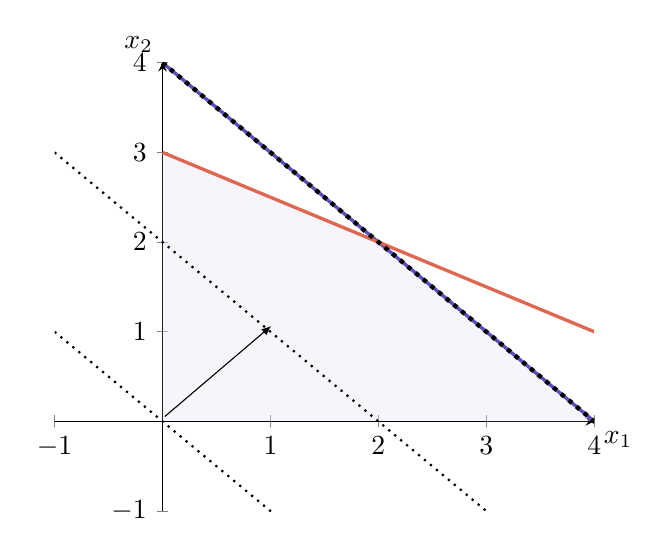
\begin{tikzpicture}
%
%
% -------------------------------------------------------
\begin{axis}[
	 axis x line=center,
  axis y line=center,
  xtick={-5,-4,...,5},
  ytick={-5,-4,...,5},
  xlabel={$x_1$},
  ylabel={$x_2$},
  xlabel style={below right},
  ylabel style={above left},
  xmin=-1,
  xmax=4,
  ymin=-1,
  ymax=4]
	legend style={at={(0.45,0.025)},anchor=south west},
]
\addplot[name path=c, domain=0:3,samples=2,color=black, style=very thin]{0};
%%%
%%%
\addplot[name path=b, domain={0:6}, color=myblue, style=very thick,samples=2]{4-x};
\addplot[name path=a, domain={0:6}, color=myred, style=very thick, samples=2]{3-0.5*x};

\addplot[fill=myblue!15,opacity=0.4] fill between [of=a and c, soft clip={domain=0:2}];
\addplot[fill=myblue!15,opacity=0.4] fill between [of=b and c, soft clip={domain=2:4}];
 
%

%	
\addplot[domain=-1:6, samples=2, color=black, dotted, thick]{-x};
\addplot[domain=-1:6, samples=2, color=black, dotted, thick]{2-x};
\addplot[domain=0:6, samples=2, color=black, dotted, ultra thick]{4-x};
\end{axis}
\draw[->] (1.4,1.2) -- (2.75,2.35);
\end{tikzpicture}
\caption{Grafisk illustration med uendeligt antal løsninger til problemet i \ref{eks:min_loes}.}
%
\label{fig:opti_loes2}
\end{figure}
\end{frame}

\begin{frame}
\frametitle{Grafisk løsning}
\begin{figure}[H]
\centering
%
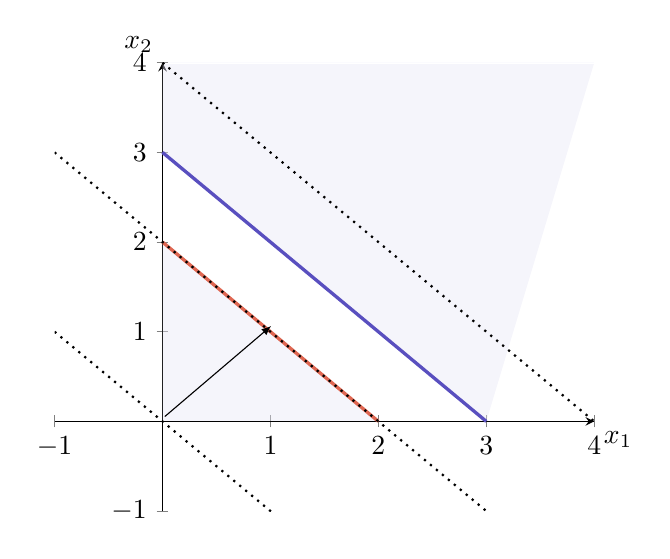
\begin{tikzpicture}
%
%
% -------------------------------------------------------
\begin{axis}[
	 axis x line=center,
  axis y line=center,
  xtick={-5,-4,...,5},
  ytick={-5,-4,...,5},
  xlabel={$x_1$},
  ylabel={$x_2$},
  xlabel style={below right},
  ylabel style={above left},
  xmin=-1,
  xmax=4,
  ymin=-1,
  ymax=4]
	legend style={at={(0.45,0.025)},anchor=south west},
]
\addplot[name path=d, domain=0:4,samples=2,color=white, style=ultra thin]{4};
\addplot[name path=c, domain=0:4,samples=2,color=black, style=ultra thin]{0};
%%%
%%%
\addplot[name path=b, domain={0:3}, color=myblue, style=very thick,samples=2]{3-1*x};
\addplot[name path=a, domain={0:2}, color=myred, style=very thick, samples=2]{2-1*x};


\addplot[fill=myblue!15,opacity=0.4] fill between [of=a and c, soft clip={domain=0:2}];
\addplot[fill=myblue!15,opacity=0.4] fill between [of=b and d, soft clip={domain=0:4}];
 

%

%	
\addplot[domain=-1:6, samples=2, color=black, dotted, thick]{-x};
\addplot[domain=-1:6, samples=2, color=black, dotted, thick]{2-x};
\addplot[domain=0:6, samples=2, color=black, dotted, thick]{4-x};
\end{axis}
\draw[->] (1.4,1.2) -- (2.75,2.35);
\end{tikzpicture}
\caption{Grafisk illustration, hvor løsningsmængden er tom til problemet i \ref{eks:min_loes3}.}
%
\label{fig:opti_loes3}
\end{figure}
\end{frame}

\begin{frame}
\frametitle{Grafisk løsning}
\begin{figure}[H]
\centering
%
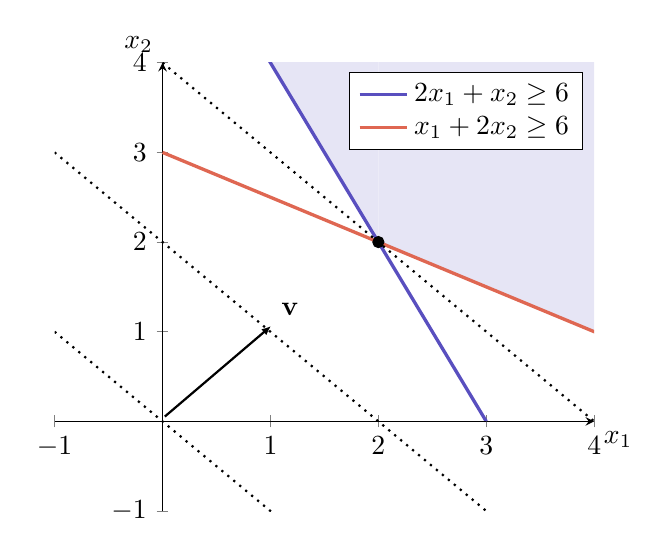
\begin{tikzpicture}
%
%
% -------------------------------------------------------
\begin{axis}[
	 axis x line=center,
  axis y line=center,
  xtick={-5,-4,...,5},
  ytick={-5,-4,...,5},
  xlabel={$x_1$},
  ylabel={$x_2$},
  xlabel style={below right},
  ylabel style={above left},
  xmin=-1,
  xmax=4,
  ymin=-1,
  ymax=4]
	legend style={at={(0.45,0.025)},anchor=south west},
]
%
%
%
%
%
\addplot[name path=b, domain={0:3}, color=myblue, style=very thick,samples=2]{6-2*x};
\addlegendentry{$2x_1+x_2 \geq 6$}
\addplot[name path=a, domain={0:6}, color=myred, style=very thick, samples=2]{3-0.5*x};
\addlegendentry{$x_1+2x_2 \geq 6$}
%%%
%%%
\addplot[name path=d, domain=0:6,samples=2,color=white, style=ultra thin]{6};
\addplot[name path=c, domain=0:3,samples=2,color=black, style=very thin]{0};



\addplot[fill=myblue!15] fill between [of=d and b, soft clip={domain=0:2}];
\addplot[fill=myblue!15] fill between [of=d and a, soft clip={domain=2:4}];
 

%

%	
\addplot[domain=-1:6, samples=2, color=black, dotted, thick]{-x};
\addplot[domain=-1:6, samples=2, color=black, dotted, thick]{2-x};
\addplot[domain=0:6, samples=2, color=black, dotted, thick]{4-x};
\addplot[mark=*] coordinates {(2,2)};
\end{axis}
\draw[thick,->] (1.4,1.2) -- (2.75,2.35) node[above right] {$\mathbf{v}$};
\end{tikzpicture}
\caption{En begrænset løsningsmængde, markeret med blå, afgrænset af lineære betingelser, hvor den optimale løsning er $\infty$ til problemet.}
%
\label{fig:opti_loes4}
\end{figure}
\end{frame}

\begin{frame}
\frametitle{Grafisk løsning}
\begin{itemize}
\item En entydig optimal løsning
\item Uendeligt mange optimale løsninger 
\item En tom løsning
\item $\infty$ eller $-\infty$ som optimal løsning  
\end{itemize}
\end{frame}

\begin{frame}
\frametitle{Standardform}
\begin{align*}
\begin{array}{lrl}
\text{Maksimér}		&z - \textbf{c}^T\textbf{x}	&	=0		\\
\text{begrænset af}	&A\textbf{x}	&=\mathbf{b},	\\
					&\mathbf{x}				&\geq \mathbf{0},
\end{array}
\end{align*}
\begin{itemize}
\item Lighedsbetingelser \\
 		Slack-variabler
\item Ikke-negativsbetingelser \\ 
		$x_i^+$ og $x_i^-$
\end{itemize}
\end{frame}

\begin{frame}
\frametitle{Dualproblemer}
\begin{align*}
\begin{array}{lrl}
\text{Maksimér}		&\textbf{c}^T\textbf{x}	& = z		\\
\text{begrænset af}	&A\textbf{x}	&\leq \mathbf{b},	\\
					&\mathbf{x}				&\geq \mathbf{0},
\end{array}
\end{align*}
%

%
%\begin{align*}
%\begin{array}{lrl}
%\text{Minimér}		&\textbf{p}^T\textbf{b}	& = v			\\
%\text{begrænset af}	&\textbf{p}^TA	&\geq (\mathbf{c})^T,	\\
%					&\mathbf{b}				&\geq \mathbf{0}
%\end{array}
%\end{align*}

\begin{align*}
\begin{array}{lrl}
\text{Minimér}		&\textbf{b}^T\textbf{p}	& = v			\\
\text{begrænset af}	&A^T \textbf{p}	&\geq \mathbf{c},	\\
					&\mathbf{p}				&\geq \mathbf{0}
\end{array}
\end{align*}
\begin{center}
\begin{tabular}{llll}
Primær  & Maksimér   & Minimér    & Dual         \\
\hline
Begræsninger & $\leq b_i$ & $\geq 0$   & Variable     \\
             & $\geq b_i$ & $\leq 0$   &              \\
             & $=b_i$     & fri        &            \\ 
\hline             
Variable     & $\geq 0$   & $\geq c_j$ & Begræsninger \\
             & $\leq 0$   & $\leq c_j$ &              \\
             & fri        & $=c_j$     &  
\end{tabular}
\end{center}
\end{frame}

\begin{frame}
\frametitle{Polyeder}
\textbf{Polyeder}
$$\mathcal{P} = \{\textbf{x} \in \R^n \mid A\mathbf{x}\geq \textbf{b}\}.$$
\\
$
\begin{array}{cc}
\begin{minipage}[b]{0.45\textwidth}
%%%%%%%%%%%%%%%%%%%%%%%%%%%%%%%%
%%% Flot graf alla Julie     %%%
%%%%%%%%%%%%%%%%%%%%%%%%%%%%%%%%
%
\begin{center}
%start tikz picture, and use the tdplot_main_coords style to implement the display 
%coordinate transformation provided by 3dplot
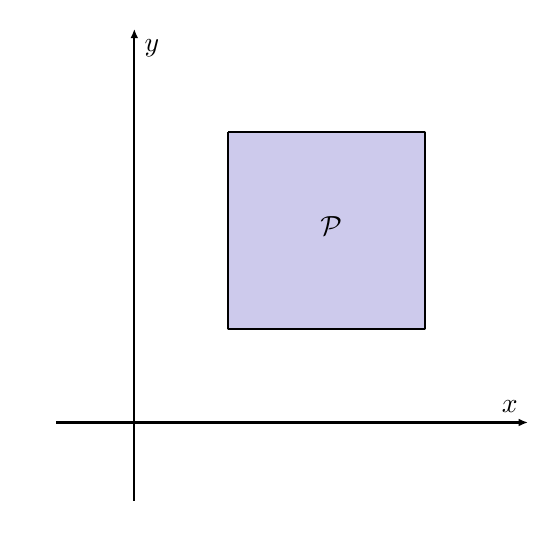
\begin{tikzpicture}[scale=5]%[scale=5,tdplot_main_coords]
%set up some coordinates 
%-----------------------
\coordinate (a) at (1.2,1.2,0.7);
\coordinate (b) at (0.7,1.2,0.7);
\coordinate (c) at (0.7,1.2,1.2);
\coordinate (d) at (1.2,1.2,1.2);
\coordinate (f) at (1.2,0.7,0.7);
\coordinate (g) at (1.2,0.7,1.2);
\coordinate (h) at (0.7,0.7,1.2);
%
%draw figure contents
%--------------------
\filldraw[fill=myblue,opacity=0.3, thick](c)--(d)--(g)--(h)--(c);
  \draw[thick](d)--(g);
  \draw[thick](d)--(c);
  \draw[thick](g)--(h);
  \draw[thick](h)--(c);
%
\draw[black] (0.91,0.96,1.2) circle (0pt) node[anchor=west] {$\mathcal{P}$};
\draw[black] (0,0,0.7) circle (0pt);
%draw the main coordinate system axes
\draw[thick,->] (0,0,0) -- (1,0,0) node[anchor=south east]{$x$};
\draw[thick] (0,0,0) -- (-0.2,0,0);
\draw[thick,->] (0,0,0) -- (0,1,0) node[anchor=north west]{$y$};
\draw[thick] (0,0,0) -- (0,-0.2,0);
\end{tikzpicture}
  \captionof{figure}{En polyede $\mathcal{P}$ markeret med blå i $\R^2$.}
  \label{fig:nej2}
\end{center}
\end{minipage}&
\begin{minipage}[b]{0.45\textwidth}
\begin{center}
%
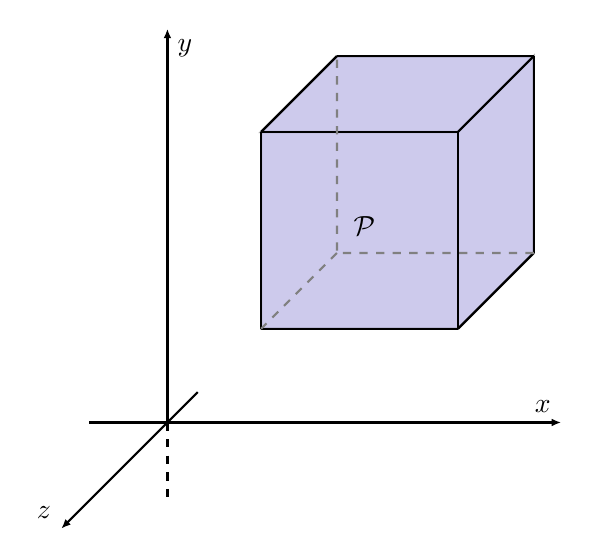
\begin{tikzpicture}[scale=5]
% Koordinater 
% -------------------------------------------------------
\coordinate (a) at (1.2,1.2,0.7);
\coordinate (b) at (0.7,1.2,0.7);
\coordinate (c) at (0.7,1.2,1.2);
\coordinate (d) at (1.2,1.2,1.2);
\coordinate (f) at (1.2,0.7,0.7);
\coordinate (g) at (1.2,0.7,1.2);
\coordinate (h) at (0.7,0.7,1.2);
%
% Figur
% -------------------------------------------------------
\filldraw[fill=myblue,opacity=0.3, thick](a)--(b)--(c)--(d)--(a)--(f)--(g)--(h)--(c)--(d)--(a);
  \draw[thick](d)--(g);
  \draw[thick](g)--(f);
  \draw[thick](f)--(a);
  \draw[thick](a)--(d);
  \draw[thick](d)--(c);
  \draw[thick](g)--(h);
  \draw[thick](c)--(b);
  \draw[thick](h)--(c);
  \draw[thick](b)--(a);
  \draw[gray, thick, dashed](f)--(0.7,0.7,0.7)--(0.7,1.2,0.7);
  \draw[gray, thick, dashed](0.7,0.7,0.7)--(0.7,0.7,1.2);
%
%
% Navngivning og prik til at gøre det pænt 
% -------------------------------------------------------
\draw[black] (0.91,0.96,1.2) circle (0pt) node[anchor=west] {$\mathcal{P}$};
% 
% 
% Koordinatssystem 
% -------------------------------------------------------
\draw[thick,->] (0,0,0) -- (1,0,0) node[anchor=south east]{$x$};
\draw[thick] (0,0,0) -- (-0.2,0,0);
\draw[thick,->] (0,0,0) -- (0,1,0) node[anchor=north west]{$y$};
\draw[thick,dashed] (0,0,0) -- (0,-0.2,0);
\draw[thick,->] (0,0,0) -- (0,0,0.7) node[anchor=south east]{$z$};
\draw[thick] (0,0,0) -- (0,0,-0.2);
%
%
\end{tikzpicture}
  \captionof{figure}{En polyede $\mathcal{P}$ markeret med blå i $\R^3$.}
  \label{fig:nej3}
\end{center}
%
\end{minipage}
\end{array}
$
\\
\textbf{Polyedre på standardform} 
$$\mathcal{P}=\{ \mathbf{x} \in \R^n  \mid  A\mathbf{x}=\mathbf{b}, \mathbf{x} \geq \mathbf{0} \},$$
\end{frame}

\begin{frame}
\frametitle{Hyperplan}
\textbf{Hyperplan}
$$\{\textbf{x} \in \R^n \mid \mathbf{a}^T \mathbf{x}=b\}$$ 
%
\textbf{Øvre halvrum}
$$\{\textbf{x} \in \R^n \mid \mathbf{a}^T \mathbf{x} \geq b\}$$ 
\textbf{Nedre halvrum}
$$\{\textbf{x} \in \R^n \mid \mathbf{a}^T \mathbf{x} \leq b\}$$ 
\end{frame}

\begin{frame}
\frametitle{Hyperplan}
\textbf{Fællesmængden}
\begin{center}
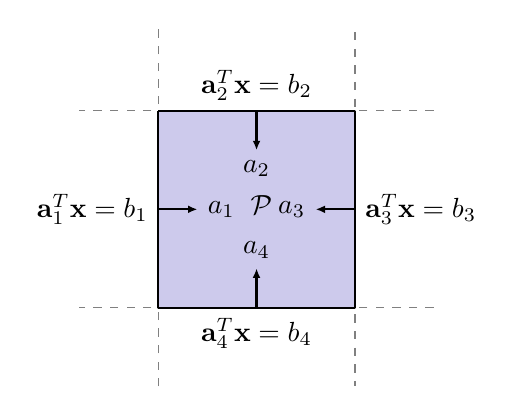
\begin{tikzpicture}[scale=5]
% Koordinater
% -------------------------------------------------------
\coordinate (c) at (0.7,1.2,1.2);
\coordinate (d) at (1.2,1.2,1.2);
\coordinate (g) at (1.2,0.7,1.2);
\coordinate (h) at (0.7,0.7,1.2);
%
% Tegning af figur og kommentarer
% -------------------------------------------------------
%
% Farve 
% -------------------------------------------------------
\filldraw[fill=myblue,opacity=0.3, thick](c)--(d)--(g)--(h)--(c);
%
% Linjer og navne
% -------------------------------------------------------
% a_1
\draw[gray,thin,dashed](0.7,0.5,1.2)--(0.7,1.41,1.2);
\draw[thick](h)--node[left]{$\mathbf{a}_1^T \mathbf{x}=b_1$} (c);
\draw[thick,->](0.7,0.95,1.2)--(0.8,0.95,1.2) node[right]{$a_1$};
%
% a_2
\draw[gray,thin,dashed](1.4,1.2,1.2)--(0.5,1.2,1.2);
\draw[thick](d)--node[above]{$\mathbf{a}_2^T \mathbf{x}=b_2$} (c);
\draw[thick,->](0.95,1.2,1.2)--(0.95,1.1,1.2) node[below]{$a_2$};
%
% a_3
\draw[gray,thin,dashed](1.2,1.4,1.2)--(1.2,0.5,1.2);
\draw[thick](d)--node[right] {$\mathbf{a}_3^T \mathbf{x}=b_3$} (g);
\draw[thick,->](1.2,0.95,1.2)--(1.1,0.95,1.2) node[left]{$a_3$};
%
% a_4  
\draw[gray,thin,dashed](1.4,0.7,1.2)--(0.5,0.7,1.2);
\draw[thick](g)--node[below]{$\mathbf{a}_4^T \mathbf{x}=b_4$} (h);
\draw[thick,->](0.95,0.7,1.2)--(0.95,0.8,1.2) node[above]{$a_4$};
%
% Navn til polyeden
% -------------------------------------------------------
\draw[black] (0.91,0.96,1.2) circle (0pt) node[anchor=west] {$\mathcal{P}$};
%
\end{tikzpicture}
\end{center}
\end{frame}


\begin{frame}
\frametitle{Konvekse hylstre }
\begin{itemize}
\item \textbf{Konveks mængde: } \\
$\lambda \textbf{u} + (1- \lambda ) \textbf{v} \in \mathcal{S}$
\item \textbf{Konveks kombination: } \\ 
Vektoren $\sum_{i=1}^{k} \lambda_i \textbf{v}_i$ af vektorerne $\textbf{v}_1, \textbf{v}_2, \ldots, \textbf{v}_k$ 
\\ $\lambda$ summeret til 1
\item \textbf{Konvekst hylster: } \\
Mængde af alle konvekse kombinationer \\
\end{itemize}
\phantom{H} \\
%%%%%%%%%%%%%%%%%%%%%%%%%%%%%%%%
%%% Flot graf alla Julie     %%%
%%%%%%%%%%%%%%%%%%%%%%%%%%%%%%%%
%
\begin{center}
% 
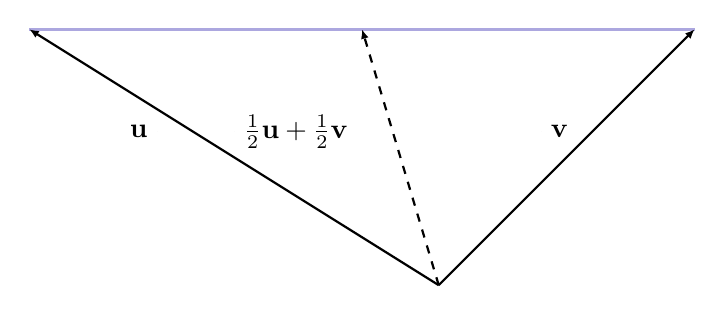
\begin{tikzpicture}[scale=6.5]
% Koordinater
% -------------------------------------------------------
\coordinate (c) at (0.7,1.2,1.2);
\coordinate (d) at (1.2,1.2,1.2);
\coordinate (g) at (1.2,0.7,1.2);
\coordinate (h) at (0.7,0.7,1.2);
\coordinate (b) at (2,1.2,1.2);
\coordinate (f) at (1.5,0.7,1.2);
%
% Tegning af vektorer
% -------------------------------------------------------
  \draw[very thick,color=myblue!50](b)--(c);  
  \draw[thick,->](f)--(b);
  \draw[thick,->](f)--(c);
  \draw[thick,->, dashed](f)--(1.35,1.2,1.2);
%
% Punkter og linje 
% -------------------------------------------------------
\filldraw[black] (0.95,1,1.2) circle (0pt) node[left] {$\mathbf{u}$};
\filldraw[black] (1.7,1,1.2) circle (0pt) node[right] {$\mathbf{v}$};
\filldraw[black] (1.1,1,1.2) circle (0pt) node[right] {$\frac{1}{2} \mathbf{u}+\frac{1}{2} \mathbf{v}$};
%
%% Koordinatssystem
%% ------------------------------------------------------
%\draw[thick,->] (0,0,-0.5) -- (1.5,0,-0.5) node[anchor=south east]{$x$};
%\draw[thick] (0,0,-0.5) -- (-0.2,0,-0.5);
%\draw[thick,->] (0,0,-0.5) -- (0,0.8,-0.5) node[anchor=north west]{$y$};
%\draw[thick] (0,0,-0.5) -- (0,-0.2,-0.5);
%%
%
\end{tikzpicture}
  \captionof{figure}{Vektorerne $\mathbf{u}$ og $ \mathbf{v}$, samt den konvekse kombination af dem, hvor $\lambda_{\textbf{u}} = \lambda_{\textbf{v}} = \frac{1}{2}$, og det konvekse hylster af vektorerne, markeret med blå.}
  \label{fig:neej2}
\end{center}
%
\end{frame}

\begin{frame}
\frametitle{Konveks funktion}
\begin{itemize}
	\item \textbf{Konveks:} 
	$$f(\lambda \textbf{u} + (1- \lambda ) \textbf{v}) \leq \lambda f( \textbf{u}) + (1- \lambda ) f(\textbf{v}) $$ 
\end{itemize}
%%%%%%%%%%%%%%%%%%%%%%%%%%%%%%%%
%%% Flot graf alla Julie     %%%
%%%%%%%%%%%%%%%%%%%%%%%%%%%%%%%%
%
\begin{center}
% 
\begin{tikzpicture}[scale=0.7]
% Koordinater
% -------------------------------------------------------

%
% Punkter og linje 
% -------------------------------------------------------
\draw[very thick, color = myblue] (1,3,0) .. controls (3,5,0) and (45,5,0) .. (7,3,0);
%\draw[very thick, color=myred] (0.1,0.5,0) .. controls (0.3,0.8,0) and (0.6,0.1,0) .. (0.7,0.4,0);

\draw[very thick, color=myred] (9,5,0) .. controls (11,8,0) and (14,1,0) .. (15,3,0);
%
%
\end{tikzpicture}
  \captionof{figure}{En konveks funktion markeret med blå, og en ikke-konveks funktion markeret med rød.}
  \label{fig:julieerkonge}
\end{center}
\begin{itemize}
\item Lokalt minimum $\rightarrow$ Globalt minimum
\end{itemize}
\phantom{H} \\
\phantom{H} \\
\end{frame}



%\begin{frame}
%\frametitle{Grafisk løsning}
%
%\begin{figure}[H]
\centering
%
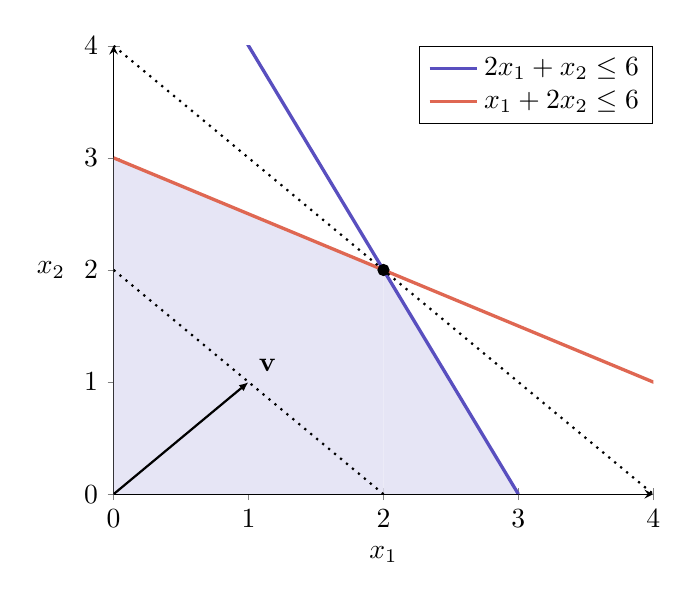
\begin{tikzpicture}%[scale=0.5]
%
%
% -------------------------------------------------------
\begin{axis}[
axis lines = left,
	xlabel = $x_1$,
	ylabel = \rotatebox{-90}{$x_2$},
  xmax=4,
  ymax=4,
	legend style={at={(1,1)},anchor=north east},
]
%%%
%%%
\addplot[name path=b, domain={0:3}, color=myblue, style=very thick,samples=2]{6-2*x};
\addlegendentry{$2x_1+x_2 \leq 6$}
\addplot[name path=a, domain={0:6}, color=myred, style=very thick, samples=2]{3-0.5*x};
\addlegendentry{$x_1+2x_2 \leq 6$}
%
\addplot[name path=c, domain=0:3,samples=2,color=black, style=very thin]{0};
%
\addplot[fill=myblue!15] fill between [of=a and c, soft clip={domain=0:2}];
\addplot[fill=myblue!15] fill between [of=b and c, soft clip={domain=2:3}];
%
%
%	
\addplot[domain=0:6, samples=2, color=black, dotted, thick]{-x};
\addplot[domain=0:6, samples=2, color=black, dotted, thick]{2-x};
\addplot[domain=0:6, samples=2, color=black, dotted, thick]{4-x};
\addplot[mark=*] coordinates {(2,2)};
\addplot[mark=none] coordinates {(0,0) (0,3)};
\addplot[mark=none, thick, ->] coordinates {(0,0) (1,1)} node[above right] {$\mathbf{v}$};
\end{axis}
\end{tikzpicture}
\end{figure}
%
%%\begin{figure}[H]
\centering
%
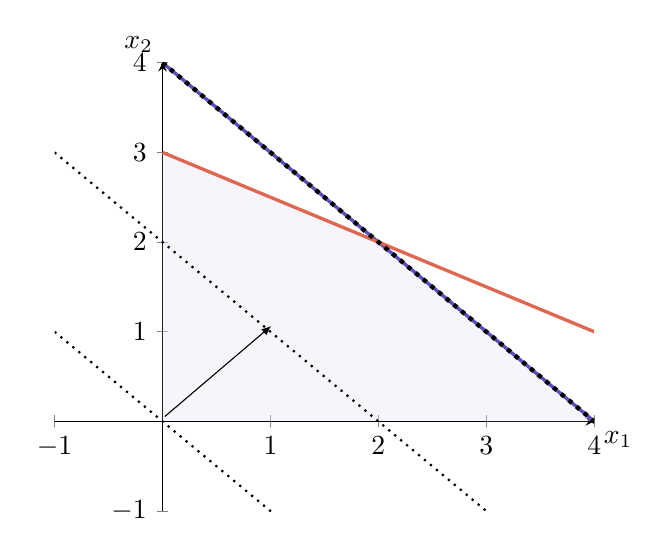
\begin{tikzpicture}
%
%
% -------------------------------------------------------
\begin{axis}[
	 axis x line=center,
  axis y line=center,
  xtick={-5,-4,...,5},
  ytick={-5,-4,...,5},
  xlabel={$x_1$},
  ylabel={$x_2$},
  xlabel style={below right},
  ylabel style={above left},
  xmin=-1,
  xmax=4,
  ymin=-1,
  ymax=4]
	legend style={at={(0.45,0.025)},anchor=south west},
]
\addplot[name path=c, domain=0:3,samples=2,color=black, style=very thin]{0};
%%%
%%%
\addplot[name path=b, domain={0:6}, color=myblue, style=very thick,samples=2]{4-x};
\addplot[name path=a, domain={0:6}, color=myred, style=very thick, samples=2]{3-0.5*x};

\addplot[fill=myblue!15,opacity=0.4] fill between [of=a and c, soft clip={domain=0:2}];
\addplot[fill=myblue!15,opacity=0.4] fill between [of=b and c, soft clip={domain=2:4}];
 
%

%	
\addplot[domain=-1:6, samples=2, color=black, dotted, thick]{-x};
\addplot[domain=-1:6, samples=2, color=black, dotted, thick]{2-x};
\addplot[domain=0:6, samples=2, color=black, dotted, ultra thick]{4-x};
\end{axis}
\draw[->] (1.4,1.2) -- (2.75,2.35);
\end{tikzpicture}
\caption{Grafisk illustration med uendeligt antal løsninger til problemet i \ref{eks:min_loes}.}
%
\label{fig:opti_loes2}
\end{figure}
%%
%%\begin{figure}[H]
\centering
%
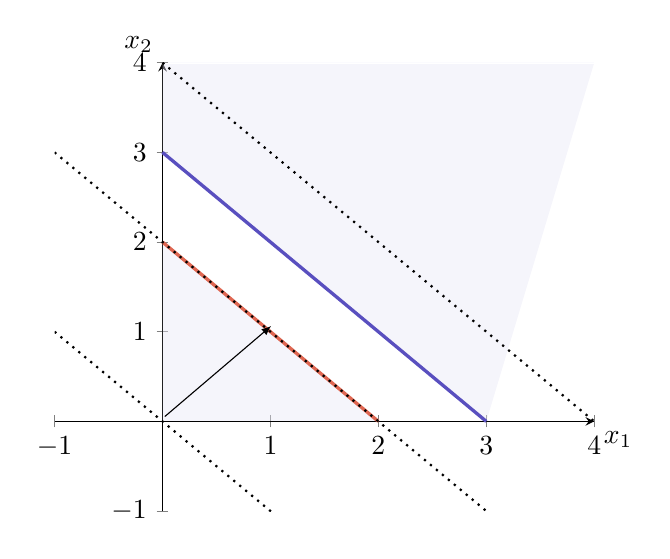
\begin{tikzpicture}
%
%
% -------------------------------------------------------
\begin{axis}[
	 axis x line=center,
  axis y line=center,
  xtick={-5,-4,...,5},
  ytick={-5,-4,...,5},
  xlabel={$x_1$},
  ylabel={$x_2$},
  xlabel style={below right},
  ylabel style={above left},
  xmin=-1,
  xmax=4,
  ymin=-1,
  ymax=4]
	legend style={at={(0.45,0.025)},anchor=south west},
]
\addplot[name path=d, domain=0:4,samples=2,color=white, style=ultra thin]{4};
\addplot[name path=c, domain=0:4,samples=2,color=black, style=ultra thin]{0};
%%%
%%%
\addplot[name path=b, domain={0:3}, color=myblue, style=very thick,samples=2]{3-1*x};
\addplot[name path=a, domain={0:2}, color=myred, style=very thick, samples=2]{2-1*x};


\addplot[fill=myblue!15,opacity=0.4] fill between [of=a and c, soft clip={domain=0:2}];
\addplot[fill=myblue!15,opacity=0.4] fill between [of=b and d, soft clip={domain=0:4}];
 

%

%	
\addplot[domain=-1:6, samples=2, color=black, dotted, thick]{-x};
\addplot[domain=-1:6, samples=2, color=black, dotted, thick]{2-x};
\addplot[domain=0:6, samples=2, color=black, dotted, thick]{4-x};
\end{axis}
\draw[->] (1.4,1.2) -- (2.75,2.35);
\end{tikzpicture}
\caption{Grafisk illustration, hvor løsningsmængden er tom til problemet i \ref{eks:min_loes3}.}
%
\label{fig:opti_loes3}
\end{figure}
%%
%%\begin{figure}[H]
\centering
%
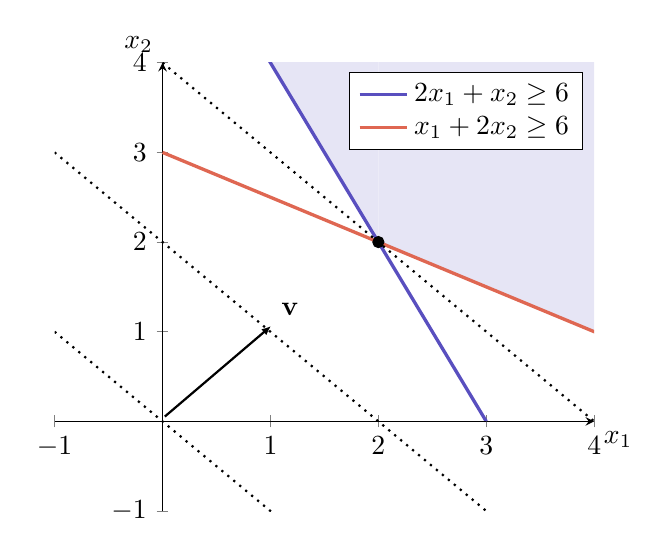
\begin{tikzpicture}
%
%
% -------------------------------------------------------
\begin{axis}[
	 axis x line=center,
  axis y line=center,
  xtick={-5,-4,...,5},
  ytick={-5,-4,...,5},
  xlabel={$x_1$},
  ylabel={$x_2$},
  xlabel style={below right},
  ylabel style={above left},
  xmin=-1,
  xmax=4,
  ymin=-1,
  ymax=4]
	legend style={at={(0.45,0.025)},anchor=south west},
]
%
%
%
%
%
\addplot[name path=b, domain={0:3}, color=myblue, style=very thick,samples=2]{6-2*x};
\addlegendentry{$2x_1+x_2 \geq 6$}
\addplot[name path=a, domain={0:6}, color=myred, style=very thick, samples=2]{3-0.5*x};
\addlegendentry{$x_1+2x_2 \geq 6$}
%%%
%%%
\addplot[name path=d, domain=0:6,samples=2,color=white, style=ultra thin]{6};
\addplot[name path=c, domain=0:3,samples=2,color=black, style=very thin]{0};



\addplot[fill=myblue!15] fill between [of=d and b, soft clip={domain=0:2}];
\addplot[fill=myblue!15] fill between [of=d and a, soft clip={domain=2:4}];
 

%

%	
\addplot[domain=-1:6, samples=2, color=black, dotted, thick]{-x};
\addplot[domain=-1:6, samples=2, color=black, dotted, thick]{2-x};
\addplot[domain=0:6, samples=2, color=black, dotted, thick]{4-x};
\addplot[mark=*] coordinates {(2,2)};
\end{axis}
\draw[thick,->] (1.4,1.2) -- (2.75,2.35) node[above right] {$\mathbf{v}$};
\end{tikzpicture}
\caption{En begrænset løsningsmængde, markeret med blå, afgrænset af lineære betingelser, hvor den optimale løsning er $\infty$ til problemet.}
%
\label{fig:opti_loes4}
\end{figure}
%
%\begin{itemize}
%\item Intro til løsninger fra afsnit 2
%%De fire punkter fra raporten (angående løsninger)
%\item Standardform.
%\item Eventuelt dualproblemer som sidebemærkning. Hvis vi skal have det med måske en bemærkning om spilteori og nulsum(slackvariable løsning for dual).
%\item Polyedre og repræsentation(herunder standardform)
%\item Det konvekse hylster.
%\item Injektiv og surjektiv (bijektiv)
%\item Lokal $\rightarrow$ Global (omkring fig 3.9)
%\end{itemize}
%\end{frame}
% Ekstremumspunkter
%
\begin{frame}
\frametitle{Hjørner}
\begin{itemize}
\item Ekstremumspunkter
\begin{itemize}
\item Ikke konveks kombination
\end{itemize}
\end{itemize}
%

\begin{figure}[h!]
  \centering
  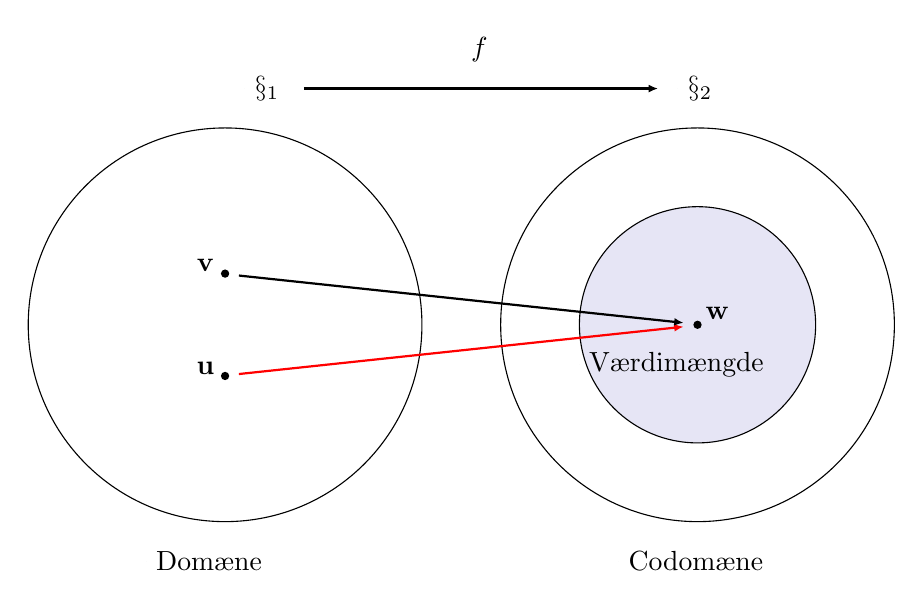
\begin{tikzpicture}
    \tikzset{punkt/.style={point, draw=black}}\draw[color=black](1,-2) circle (2.5);
	\draw[color=black](7,-2) circle (2.5);  
	\draw[color=black, fill=myblue!15](7,-2) circle (1.5);  
%Punkter
	\draw  node[fill,circle,inner sep=0pt,minimum size=3pt] at (1,-2.65)  (v1) {};
	\draw  node[fill,circle,inner sep=0pt,minimum size=3pt] at (1,-1.35)  (v2) {};
	\draw  node[fill,circle,inner sep=0pt,minimum size=3pt] at (7,-2)  (v3) {};

%Labels
	\draw  node at (0.75,-2.55)  {$\textbf{u}$};
	\draw  node at (0.75,-1.25)  {$\textbf{v}$};
	\draw  node at (7.25,-1.85)  {$\textbf{w}$};
	
	
	
	%Navn på cirklerne 
	\draw[black, fill=black] (1.25,1) circle (0pt) node[anchor=west] {$\S_1$};    
	\draw[black, fill=black] (6.75,1) circle (0pt) node[anchor=west] {$\S_2$};
	%Navn på punkter 

	\draw[black, fill=black] (4,1.5) circle (0pt) node[anchor=west] {$f$};
	
	\draw [->,thick, draw=black] (2,1) -- (6.5,1);

	 \draw [->, thick, draw=red] ([xshift=5pt, yshift=-1pt]v1.north) -- ([xshift=-5pt, yshift=1pt]v3.south);
     \draw [->, thick, draw=black] ([xshift=5pt, yshift=1pt]v2.south) -- ([xshift=-5pt, yshift=-1pt]v3.north);


	\draw[black, fill=black] (0,-5) circle (0pt) node[anchor=west] {Domæne};
	\draw[black, fill=black] (6,-5) circle (0pt) node[anchor=west] {Codomæne};
	\draw[black, fill=black] (5.5,-2.5) circle (0pt) node[anchor=west] {Værdimængde};    
	%Streger mellem punkterne
  \end{tikzpicture}
  \caption{En funktion fra $\S_1$ til $\S_2$, hvor $f(\textbf{v})=\textbf{w}$ og f$(\textbf{u})=\textbf{w}$. }
  \label{fig:afbild}
\end{figure}
%
%
%    \node[punkt] at (-4,0.5)      (v1){$v_1$};
%    \node[punkt] at (-2,0.5)      (v2){$v_2$};
%    \node[punkt] at (-4,-1.5)     (v3){$v_3$};
%    \node[punkt] at (-2,-1.5)     (v4){$v_4$};
%    \node at (-3,2)     (v){$K_{4}$};
%
%
%    \node[punkt] at (4.6,-0.2)      (k1){$v_3$};
%    \node[punkt] at (1.4,-0.2)      (k2){$v_2$};
%    \node[punkt] at (2,-2)     (k3){$v_4$};
%    \node[punkt] at (4,-2)     (k4){$v_5$};
%    \node[punkt] at (3,1)      (k5){$v_1$};
%    \node at (3,2)      (k){$K_{5}$};
%
%
%
%
%
%    \draw [-, thick, draw=black] (v1) -- (v2);
%    \draw [-, thick, draw=black] (v1) -- (v3);
%    \draw [-, thick, draw=black] (v1) -- (v4);
%    \draw [-, thick, draw=black] (v2) -- (v3);
%    \draw [-, thick, draw=black] (v2) -- (v4);
%    \draw [-, thick, draw=black] (v3) -- (v4);
\end{frame}
%
% Hjørnepunkt
%
\begin{frame}
\frametitle{Hjørner}
\begin{itemize}
\item Hjørnepunkter
\begin{itemize}
\item Alene i fællesmængde for $\mathcal{P}$ og hyperplan.
\end{itemize}
\end{itemize}
%
\begin{figure}[h!]
  \centering
  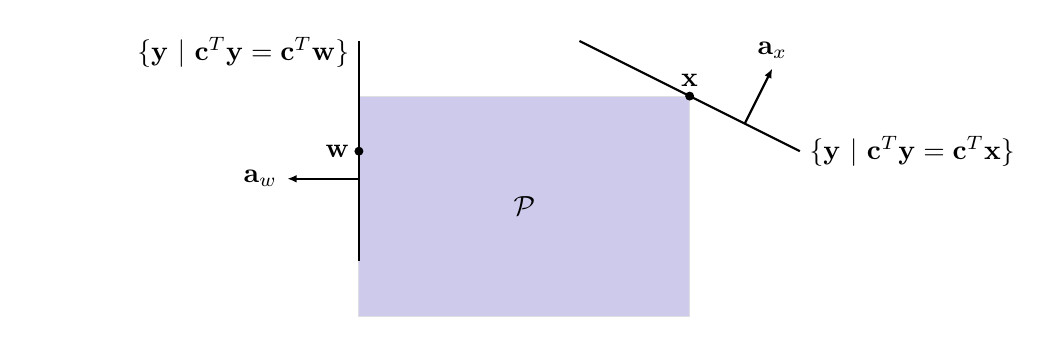
\begin{tikzpicture}[scale=0.7]
    \tikzset{punkt/.style={point, draw=black}}
%
%
% Koordinater
% -------------------------------------------------------
\coordinate (y) at (1,4);
\coordinate (x) at (3,3);
\coordinate (z) at (5,2);
\coordinate (v) at (-3,4);
\coordinate (w) at (-3,2);
\coordinate (u) at (-3,0);
%    
% Punkter
% -------------------------------------------------------
	\node at (3,3)	(1){};
	\node at (-3,3)	(4){};
	\node at (3,-1)	(2){};
	\node at (-3,-1) (3){};
% 
% Firkant 
% -------------------------------------------------------
	\filldraw[mygrey, fill=myblue!30] (2) rectangle (4);
	\node at (0,1) (P){$\mathcal{P}$};
%	
% Punkter og tilhørende tekst
% -------------------------------------------------------
	\filldraw [black] (5,2) circle (0pt) node[right] {$ \{ \mathbf{y} \text{  } | \text{  } \mathbf{c}^T \mathbf{y} = \mathbf{c}^T \mathbf{x} \}$};
	\filldraw [black] (x) circle (2pt) node[above] {$\mathbf{x}$};
	\filldraw [black] (-3,3.8) circle (0pt) node[left] {$ \{ \mathbf{y} \text{  } | \text{  } \mathbf{c}^T \mathbf{y} = \mathbf{c}^T \mathbf{w} \}$};
	\filldraw [black] (w) circle (2pt) node[left] {$\mathbf{w}$};
%
% Streger mellem punkterne 
% -------------------------------------------------------
	\draw[-,black, thick] (v) -- (w) -- (u);
	\draw[-,black, thick] (y) -- (x);
	\draw[-,black, thick] (x) -- (z);
	\draw[->,black, thick] (-3,1.5) -- (-4.3,1.5) node[left]  {$\mathbf{a}_w$};
	\draw[->,black, thick] (4,2.5) -- (4.5,3.5) node[above] {$\mathbf{a}_x$};
%
\filldraw [black] (-9,2) circle (0pt);
%
  \end{tikzpicture}
  \caption{En polyede $\mathcal{P}$, hvor $\textbf{x}$ er et hjørnepunkt, da hyperplanet kun rammer $\mathcal{P}$ i $\mathbf{x}$. Vektoren $\textbf{w}$ er i modsætning ikke hjørnepunkt, da hyperplanet rammer $\mathcal{P}$ i flere punkter end $\mathbf{w}$.}
  \label{fig:julieermegaseeeeeeeeeej}
\end{figure}
%
\end{frame}
%
% Basale mulige løsninger
%
\begin{frame}
\frametitle{Hjørner}
\begin{itemize}
\item Basale mulige løsninger
\begin{itemize}
\item Alle betingelser opfyldt og $n$ aktive betingelser
\end{itemize}
\end{itemize}
%
\begin{center}
%
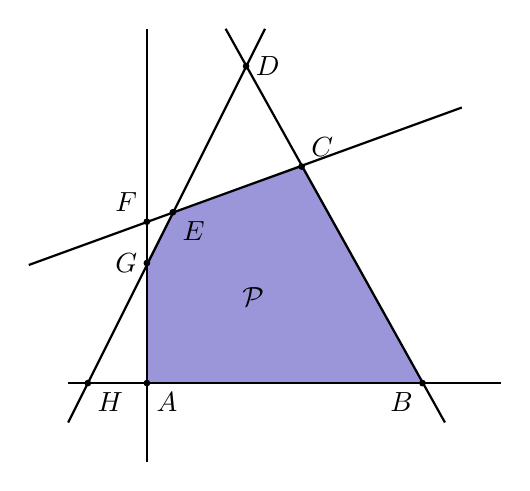
\begin{tikzpicture}[scale=5]
%
% Koordinater
% -------------------------------------------------------
\coordinate (a) at (0,0,0); 
\coordinate (b) at (0.7,0,0); 
\coordinate (c) at (0.393,0.55,0); 
\coordinate (d) at (0.252,0.805,0);
\coordinate (e) at (0.066,0.434,0);
\coordinate (f) at (0,0.41,0);
\coordinate (g) at (0,0.305,0);
\coordinate (h) at (-0.15,0,0); 
%
% Farvning
% -------------------------------------------------------
\filldraw[fill=myblue,opacity=0.6](a)--(b)--(c)--(e)--(g)--(a);
  \draw[thick](-0.2,-0.1,0)--(0.3,0.9,0); % n -> d  
  \draw[thick](0.2,0.9,0)--(0.757,-0.1,0); % d -> b
  \draw[thick](-0.3,0.3,0)--(0.8,0.7,0); % f -> c
% 
%
% Punkterne 
% -------------------------------------------------------
\filldraw [black] (a) circle (0.2pt) node[anchor=north west] {$A$};
\filldraw [black] (b) circle (0.2pt) node[anchor=north east] {$B$};
\filldraw [black] (c) circle (0.2pt) node[anchor=south west] {$C$};
\filldraw [black] (d) circle (0.2pt) node[anchor=west] {$D$};
\filldraw [black] (e) circle (0.2pt) node[anchor=north west] {$E$};
\filldraw [black] (f) circle (0.2pt) node[anchor=south east] {$F$};
\filldraw [black] (g) circle (0.2pt) node[anchor=east] {$G$};
\filldraw [black] (h) circle (0.2pt) node[anchor=north west] {$H$};
%
% 
\filldraw [black] (0.27,0.17,0) circle (0pt) node[above] {$\mathcal{P}$};
% 
% Koordinatssystem 
% -------------------------------------------------------
\draw[thick] (0,0,0) -- (0.9,0,0);
\draw[thick] (0,0,0) -- (-0.2,0,0);
\draw[thick] (0,0,0) -- (0,0.9,0);
\draw[thick] (0,0,0) -- (0,-0.2,0);
%
\end{tikzpicture}
  \captionof{figure}{Punkterne $A,B,C,D,E,F,G$ og $H$ er basal løsninger, hvoraf $A,B,C,E$ og $G$ alle er basal mulige løsninger.}
  \label{fig:fig:basale}
\end{center}
%
\end{frame}
%
% Ækvivalens af hjørner
% (b) -> (a)
%
\begin{frame}
\frametitle{Ækvivalens mellem hjørner}
\begin{itemize}
\item Hjørnepunkt $\rightarrow$ ekstremumspunkt
\begin{itemize}
%
\item Hjørnepunkt giver
\end{itemize}
%
\centering
$
\begin{array}{ll}
\textbf{c}^T\textbf{u} < \textbf{c}^T\textbf{v}, &\textbf{v}\in \mathcal{P}, \textbf{v} \neq \textbf{u}\\
\textbf{c}^T\textbf{u} < \textbf{c}^T(\lambda\textbf{v} + (1-\lambda)\textbf{w}), &\textbf{v},\textbf{w} \in \mathcal{P}
\end{array}
$
%
\begin{itemize}
\item $\textbf{u}$ er ikke en konveks kombination
\end{itemize}
\end{itemize}
%
\end{frame}
%
% (a) -> (c)
%
\begin{frame}
\frametitle{Ækvivalens mellem hjørner}
\begin{itemize}
\item Ekstremumspunkt $\rightarrow$ basal mulig løsning
%
\begin{itemize}
\item Under $n$ aktive lineært uafhængige betingelser
\item $\textbf{d}$ ortogonal på underrummet
\item Lille $\varepsilon$
\end{itemize}

%
\centering
$
\begin{array}{ll}
\textbf{a}_i^T(\textbf{u} \pm \varepsilon \textbf{d}) > b_i, &i\notin I\\
\end{array}
$
\begin{itemize}
\item $\textbf{u}$ konveks kombination
\end{itemize}
\end{itemize}
%
\end{frame}
%
% (c) -> (b)
%
\begin{frame}
\frametitle{Ækvivalens mellem hjørner}
\begin{itemize}
\item Basal mulig løsning $\rightarrow$ hjørnepunkt
\begin{itemize}
\item Lav $\textbf{c} = \sum_{i\in I} \textbf{a}_i$
\end{itemize}
%
\begin{align*}
\textbf{c}^T\textbf{u} &= \sum_{i\in I} \textbf{a}_i^T\textbf{u} = 
 \sum_{i\in I} b_i\\
\textbf{c}^T\textbf{v} &= \sum_{i\in I} \textbf{a}_i^T\textbf{v} > 
 \sum_{i\in I} b_i, &\textbf{v}\in \mathcal{P}, \textbf{v} \neq \textbf{u}
\end{align*}
%
\begin{itemize}
\item $\textbf{u}$ alene i hyperplanet $\textbf{c}^T\textbf{x} = \sum_{i\in I} b_i$
\end{itemize}
\end{itemize}
\end{frame}
%
%
%
\begin{frame}
\frametitle{Løsning i hjørne}
\begin{itemize}
\item Mindst ét ekstremumspunkt og optimal løsning
\item $Q$ indeholder optimale løsninger i $\mathcal{P}$
\item $\textbf{u}$ optimale løsninger til $\mathcal{P}$ og ekstremumspunkt til $Q$
\item Antag $\textbf{u}$ ikke er ekstremumspunkt til $\mathcal{P}$
%
\begin{align*}
\textbf{u} &= \lambda\textbf{v} + (1-\lambda)\textbf{w}\\
\textbf{c}^T\textbf{v} &\geq y, \textbf{v} \in \mathcal{P}\\
\textbf{c}^T\textbf{v} &= \textbf{c}^T\textbf{w} = y
\end{align*}
%
\item $\textbf{u}$ ikke ekstremumspunkt i $Q$
%
\end{itemize}
\end{frame}
\begin{frame}
Lad et lineært optimeringsproblem være, at $\textbf{c}^T \textbf{x}$ skal minimeres over et polyeder $\mathcal{P}$. 
Antag, at der i $\mathcal{P}$ er mindst ét ekstremumspunkt. 
Så er den optimale omkostning lig $- \infty$, eller også findes et optimalt ekstremumspunkt.
\end{frame}

\begin{frame}
\begin{itemize}
\item $k$ lineært uafhængige betingelser aktive ved et element $\textbf{v}\in \mathcal{P} \rightarrow rank(v)=k < n$. Altså et ægte underum.
\item $I = \{ i \mid \textbf{a}^T_i \textbf{v} = b_i \}$, hvor $\textbf{a}^T_i$ er den $i$'te række af $A$.
\item  Der kan altså vælges en ikke-nulvektor $\textbf{d} \in \mathcal{R}^n$ der er ortogonal med hver række i $A$.
\item Halvlinjen $\textbf{u}=\textbf{v}+ \lambda \textbf{d}$, hvor $\lambda$ er positiv opfylder dermed, at $\textbf{a}^T_i \textbf{u} = b_i$
\end{itemize}
\end{frame}
\begin{frame}
\begin{itemize}
\item Hvis $\textbf{u}$ ikke er uendelig, er der således en grænseværdi, hvor den udgår fra $\mathcal{P}$.
\item Der findes så en vektor/punkt $\textbf{u}$ med højere rang end $\textbf{v}$, således $\textbf{c}^T \textbf{u} \leq \textbf{c}^T \textbf{v}$.
\item Forsættes indtil den basale mulig løsning $\textbf{w}$ findes, hvor $\textbf{w}=rank(n)$ og $\textbf{c}^T \textbf{w} \leq \textbf{c}^T \textbf{v}$.
\end{itemize}
\end{frame}
\begin{frame}
\begin{itemize}
\item En løsning $w*$ skal nu findes, hvorom det gælder, at $\textbf{c}^T\textbf{w}*<\textbf{c}^T \textbf{w}_i$.
\item Da $\textbf{c}^T \textbf{w}_i \leq \textbf{c}^T \textbf{v}$, er $\textbf{w}*$ en optimal løsning.
\item Det centrale er derfor brugen af ortogonalitet, samt en optimal værdi af $\lambda$ således vi ender i et hjørnepunkt.
\end{itemize}
\end{frame}

%\begin{frame}
%\begin{itemize}
%\item Metoden starter i origo.
%\item Basen er det punkt vi er i.
%\item Den største negative værdi identificeres, da det er punktet der vil forbedre løsningen hurtigst. Flyttes af kanterne. 
%\item Koeficienter ved pivotering bruges til at holde os indenfor polyedraet.
%\item  Dermed sikres en løsning, hvor en variabel bliver så stor som mulig uden at bryde grænserne, hvilket er et hjørnepunkt.
%\item Gentages til nabohjørnepunkt.
%\end{itemize}
%\end{frame}



%\begin{frame}
%\frametitle{Hjørner}
%\begin{itemize}
%\item \textbf{$nr. 5$}
%\item Bevis for løsninger i hjørnepunkter (3.9)
%\item Outro $\rightarrow$ hjørnepunkter og simplex
%\end{itemize}
%\end{frame}

\section{Simplexmetoden}
\begin{frame}
\centering
\Huge
Simplexmetoden
\end{frame}
%
\begin{frame}
\frametitle{Simplexmetoden}
\begin{itemize}
\item Finder en optimal løsning, så længe der findes mindst én basal mulig løsning
\item Anvender reduceret omkostning til at forbedre løsning
\item Problemer kan opstå
\begin{itemize}
\item Degenerering
\end{itemize}
\item 3 forskellige implementeringer.
\end{itemize}
\end{frame}
%
%     %%%%%%%%%%%%%%%%%%%%%%%%%%%%%%%%%%%%%
%     %%%%%                           %%%%%
%     %%%%%      Person nummer 6      %%%%%
%     %%%%%                           %%%%%
%     %%%%%%%%%%%%%%%%%%%%%%%%%%%%%%%%%%%%%
%
%\begin{frame}
%\frametitle{Simplexmetoden}
%\begin{itemize}
%\item Hvordan simplex afsøger hjørnepunkter.
%\item \textbf{$nr. 6$}
%\item Implementationer af simplex(tænker kort gennemgang af forskelle)
%\item Gennemgang af fuld tabelimplementering (mere udførligt (eksempel)).
%\item Lexicografi til valg af pivoteringsmetode.
%\item Kompleksitet som udgangspunkt for valg af metode.
%\item Afrunding / konklusion?!
%\end{itemize}
%\end{frame}
%
\begin{frame}
\frametitle{Implementeringer}
\begin{itemize}
\item Den naive implementering 
	\begin{itemize}
	% \item Høj tidspkompleksitet 
	\item Løser to lineær ligningssystemer
	\end{itemize}
\item Den reviderede implementering 
	\begin{itemize}
	\item $B^{-1}$ opdateres ved hver iteration
	\end{itemize}
\item Fuld-tabel implementeringen
	\begin{itemize}
	\item Simplextabel opdateres ved hver iteration
	\end{itemize} 
\end{itemize}
\end{frame}

\begin{frame}
\frametitle{Fuld-tabel implementeringen}
\begin{itemize}
\item Simplextabel 
\item Pivotering
\end{itemize}
\begin{align*}
\begin{blockarray}{ccccccccccc}
x_1 & x_2 & \cdots & x_n & \textcolor{blue}{s_1} & \textcolor{blue}{s_2} &  \textcolor{blue}{\cdots} & \textcolor{blue}{s_m} & z & b \\
\begin{block}{[cccc|ccccc|c]c}
a_{1,1} & a_{1,2} & \cdots & a_{1,n} & 1 & 0 & \cdots & 0 & 0 & b_1 \\
a_{2,1} & a_{2,2} & \cdots & a_{2,n} & 0 & 1 & \cdots & 0 & 0 & b_2 \\
\vdots & \vdots & \ddots & \vdots & \vdots & \vdots & \ddots & \vdots & \vdots & \vdots \\
a_{m,1} & a_{m,2} & \cdots & a_{m,n} & 0 & 0 & \cdots  & 1  & 0 & b_{m}\\
\cline{1-10}
-c_1 & -c_2 & \cdots & -c_n & 0 & 0 & \cdots & 0 & 1 & z\\
\end{block}
\end{blockarray}.
\end{align*}
\end{frame}

\begin{frame}
\frametitle{Pivoteringsløkker}
\begin{itemize}
\item Lexicografi
	\begin{itemize}
	\item $\mathbf{u}$ er lexicografisk større $\textbf{u} >^L \textbf{v}$
	\item $\mathbf{u}$ er lexicografisk mindre $ \textbf{u} <^L \textbf{v}$
	\end{itemize}
\item Lexicografiske metode 
\end{itemize}
\end{frame}

\begin{frame}
\frametitle{Kompleksitet}
%som udgangspunkt for valg af metode.
\begin{itemize}
\item Den naive implementering 
	\begin{itemize}
	% \item Høj tidspkompleksitet 
	\item $O(m^3)$ 
	\end{itemize}
\item Den reviderede implementering 
	\begin{itemize}
	\item $O(mn)$
	\end{itemize}
\item Fuld-tabel implementeringen
	\begin{itemize}
	\item $O(mn)$
	\end{itemize} 
\item Typisk efter $O(m)$
\end{itemize}
\end{frame}
\section{Procesanalyse}
\begin{frame}{Procesanalyse}
%\frametitle{Proces(hvis vi gider)}
\begin{itemize}
\item Er der mere tid? Har Horia lyst til at høre på det? Nej
\item Projektarbejde i cornaens tidsalder.
\item En flot tegning
\end{itemize}
\end{frame}


\bibliographystyle{apalike}
\nocite{*}
% \begin{frame}{References}
% \tiny\bibliography{bib/bibliography}
% \end{frame}

\end{document}